\documentclass{article}

\usepackage{subcaption}

\usepackage{arxiv}

\usepackage[utf8]{inputenc} % allow utf-8 input
\usepackage[T1]{fontenc}    % use 8-bit T1 fonts
\usepackage{hyperref}       % hyperlinks
\usepackage{url}            % simple URL typesetting
\usepackage{booktabs}       % professional-quality tables
\usepackage{amsfonts}       % blackboard math symbols
\usepackage{nicefrac}       % compact symbols for 1/2, etc.
\usepackage{microtype}      % microtypography
\usepackage{lipsum}		% Can be removed after putting your text content
\usepackage{graphicx}
\usepackage{natbib}
\usepackage{doi}
\usepackage{amsmath}
\title{Crowds Are Mass: Rethinking Evaluation for Crowd Density Forecasting}

%\date{September 9, 1985}	% Here you can change the date presented in the paper title
%\date{} 					% Or removing it

\author{ \href{https://orcid.org/0000-0000-0000-0000}{\includegraphics[scale=0.06]{orcid.pdf}\hspace{1mm}Khalid AlAmoudi} \\
	Department of Computer Science and AI\\
    University of Jeddah\\
	Jeddah, Saudi Arabia \\
	\texttt{KALAAMOUDI@uj.edu.sa} \\
	%% examples of more authors
	\And
	\href{https://orcid.org/0000-0000-0000-0000}{\includegraphics[scale=0.06]{orcid.pdf}\hspace{1mm} Alala Bahamid} \\
	SDAIA-KFUPM\\
	JRC for Artificial Intelligence\\
	Dhahran, Saudi Arabia \\
	\texttt{alala.bahamid@kfupm.edu.sa} \\
	%% \AND
	%% Coauthor \\
	%% Affiliation \\
	%% Address \\
	%% \texttt{email} \\
	%% \And
	%% Coauthor \\
	%% Affiliation \\
	%% Address \\
	%% \texttt{email} \\
	%% \And
	%% Coauthor \\
	%% Affiliation \\
	%% Address \\
	%% \texttt{email} \\
}

% Uncomment to remove the date
%\date{}

% Uncomment to override  the `A preprint' in the header
\renewcommand{\headeright}{KFUPM}
\renewcommand{\undertitle}{KFUPM}


%%% Add PDF metadata to help others organize their library
%%% Once the PDF is generated, you can check the metadata with
%%% $ pdfinfo template.pdf
 \hypersetup{
pdftitle={Crowds Are Mass: Rethinking Evaluation for Crowd Density Forecasting},
pdfauthor={Khalid AlAmoudi, Alala Bahamid},
}

\begin{document}
\maketitle
\begin{abstract}
A density map says how many people are in a scene and where they are. Normalizing it before scoring removes the headcount. We check what this means for crowd density forecasting: multiplying a true map by 100 still receives the score of a perfect forecast. Count error has the opposite limit: a uniform map can get the total right while losing the crowd's location. We use unbalanced optimal transport to score both errors in one comparison, with an explicit price for unmatched people. On 1{,}448 Grand Central Station clips, Stream-CDF ranks fourth of five under normalized divergence and first under transport, in every crowd-dynamics stratum. The strata also expose a rise in CrowdMAC's count error that the pooled result hides. A second recording shows smaller, scene-dependent differences. The measure changes which forecast looks best.
\end{abstract}
\keywords{crowd density forecasting \and evaluation metrics \and stratified
evaluation \and spatiotemporal forecasting \and crowd safety}

\section{Introduction}
\label{sec:intro}

To hold a train or open another exit, an operator needs to know how many people will be somewhere, and when. Crowd density forecasting asks this question from a sequence of past density maps \cite{niu2020}.

The map already contains both parts of the answer. It sums a unit-mass Gaussian at every annotated head \cite{lempitsky2010}, so its total is the headcount and its shape is the crowd's arrangement. A forecast can get either part wrong: the right crowd in the wrong place, or the right arrangement with too few people.

The reported metrics can miss headcount error. Jensen--Shannon and KL divergence compare maps after dividing each by its own total \cite{minoura2020, fujii2025}. Fifty people and five hundred people arranged the same way become the same distribution. Adding count error reveals the missing headcount, but leaves two separate scores: one can miss count error, the other ignores placement. Neither says how to weigh an improvement in one against a failure in the other.

Unbalanced optimal transport offers a joint comparison \cite{chizat2018}. It charges for moving mass and for leaving mass unmatched. Entropic Sinkhorn iterations make the comparison practical \cite{cuturi2013}, and debiasing removes the error floor introduced by regularization \cite{feydy2019}. We use this existing machinery to ask three questions:

\begin{itemize}
    \item[\textbf{RQ1}] Do the reported divergences detect headcount error?
    \item[\textbf{RQ2}] Can one measure score count and placement at test-set scale?
    \item[\textbf{RQ3}] How do metric choice and crowd dynamics change model assessment?
\end{itemize}

The last question needs more than a pooled score. Small changes and rapid dispersal pose different forecasting problems, yet an average can hide the difference \cite{oakden2020, wang2026}. We therefore group clips by how much their true headcount changes over the forecast horizon.

We test the questions on 1{,}448 Grand Central Station clips. Controlled cases check what each measure detects. Five forecasters then show whether that difference changes their ranking, both overall and within each dynamics stratum. A second, indoor recording and a sweep of the transport exchange rate check how far the result holds.

\section{Related Work}
\label{sec:related-work}

\subsection{Crowd Density Estimation and Forecasting}
\label{sec:related-density}

Density regression represents a count as the integral of a map \cite{lempitsky2010}. Multi-column and dilated networks made it a standard approach to counting from images \cite{zhang2016, li2018}. Later losses addressed the limits of pixel regression: Bayesian loss supervises maps through a posterior over annotated points \cite{ma2019}, while DM-Count combines count error with transport between normalized maps \cite{wang2020}. DM-Count is the closest use of transport to ours. Its transport term compares shape, with a separate term for count. We transport unnormalized maps, so placement and unmatched mass enter the same solve.

Counting benchmarks report mean absolute and squared count error \cite{wang2020}, often broken down by density level \cite{wang2021}. Forecasting uses the same representation but commonly evaluates its normalized shape.

Niu et al. introduced crowd forecasting as an over-crowdedness alert task \cite{niu2020}. Patch-based forecasting uses KL divergence on normalized maps \cite{minoura2020}; CrowdMAC reports average and final Jensen--Shannon divergence \cite{fujii2025}. Related work predicts indoor density over multiple steps \cite{mscdp2023}, models density and velocity with diffusion \cite{morales2025}, or studies crowd-crush risk through density representations \cite{vtcrowdnet2026}. Trajectory methods instead forecast individual paths \cite{alahi2016social, gupta2018socialgan}. They require positions and identities, face occlusion, and score displacement rather than the resulting density field. These approaches leave open how to evaluate count and placement together in a forecast map.

\subsection{Optimal Transport for Density Representations}
\label{sec:related-ot}

Optimal transport measures the cost of moving one map onto another. Unlike binwise divergence, it accounts for how far mass must move. Entropic regularization makes the solve efficient \cite{cuturi2013}, but introduces a bias even when the maps agree. Sinkhorn debiasing removes this floor \cite{feydy2019}; Peyr\'e and Cuturi give a broader treatment \cite{peyre2019}.

Classical transport requires equal mass. Crowd forecasts need not have the correct headcount, so we use unbalanced transport, which relaxes that constraint and charges for unmatched mass \cite{chizat2018}. The formulation is established. Our contribution is to test what changes when it is used to evaluate crowd forecasts.

\subsection{Evaluation and Hidden Stratification}
\label{sec:related-evaluation}

Hidden stratification describes failures on meaningful subgroups that an aggregate score conceals \cite{oakden2020}. In forecasting, recent work finds larger errors during transitions \cite{wang2026}, evaluates predictions through the decisions they support \cite{namazi2026}, and calls for diagnostics by regime \cite{phungtua2026}.

Weather forecasting shows a related problem: pixel losses can penalize displacement twice and favor smooth output, motivating losses that separate amplitude from decorrelation \cite{doublepenalty2025}. Precipitation nowcasting is a close analogue to crowd forecasting: a dense field, changing mass, and a strong persistence baseline. Its evaluation separates intensity levels because an aggregate can reward smooth forecasts \cite{ravuri2021}. We apply the same reasoning to crowd dynamics and examine the measure itself.

\section{Mass-Aware Evaluation of Crowd Forecasts}
\label{sec:motivation}

\subsection{What Normalization Removes}
\label{sec:motivation-normalized}

The reported Jensen--Shannon and KL implementations normalize their KL arguments by their sums \cite{minoura2020, fujii2025}. Maps that differ only in scale then become identical in these comparisons. This makes proportional headcount errors invisible; CrowdMAC's JS implementation has an additional mixture detail described in Section~\ref{sec:setup-metrics}.

Figure~\ref{fig:problem} shows the two limits. Normalized divergence misses a change in count when the arrangement is fixed. Count error misses a change in arrangement when the total is fixed. Reporting both exposes both errors, but does not give a joint comparison.

\begin{figure*}[t]
  \centering
  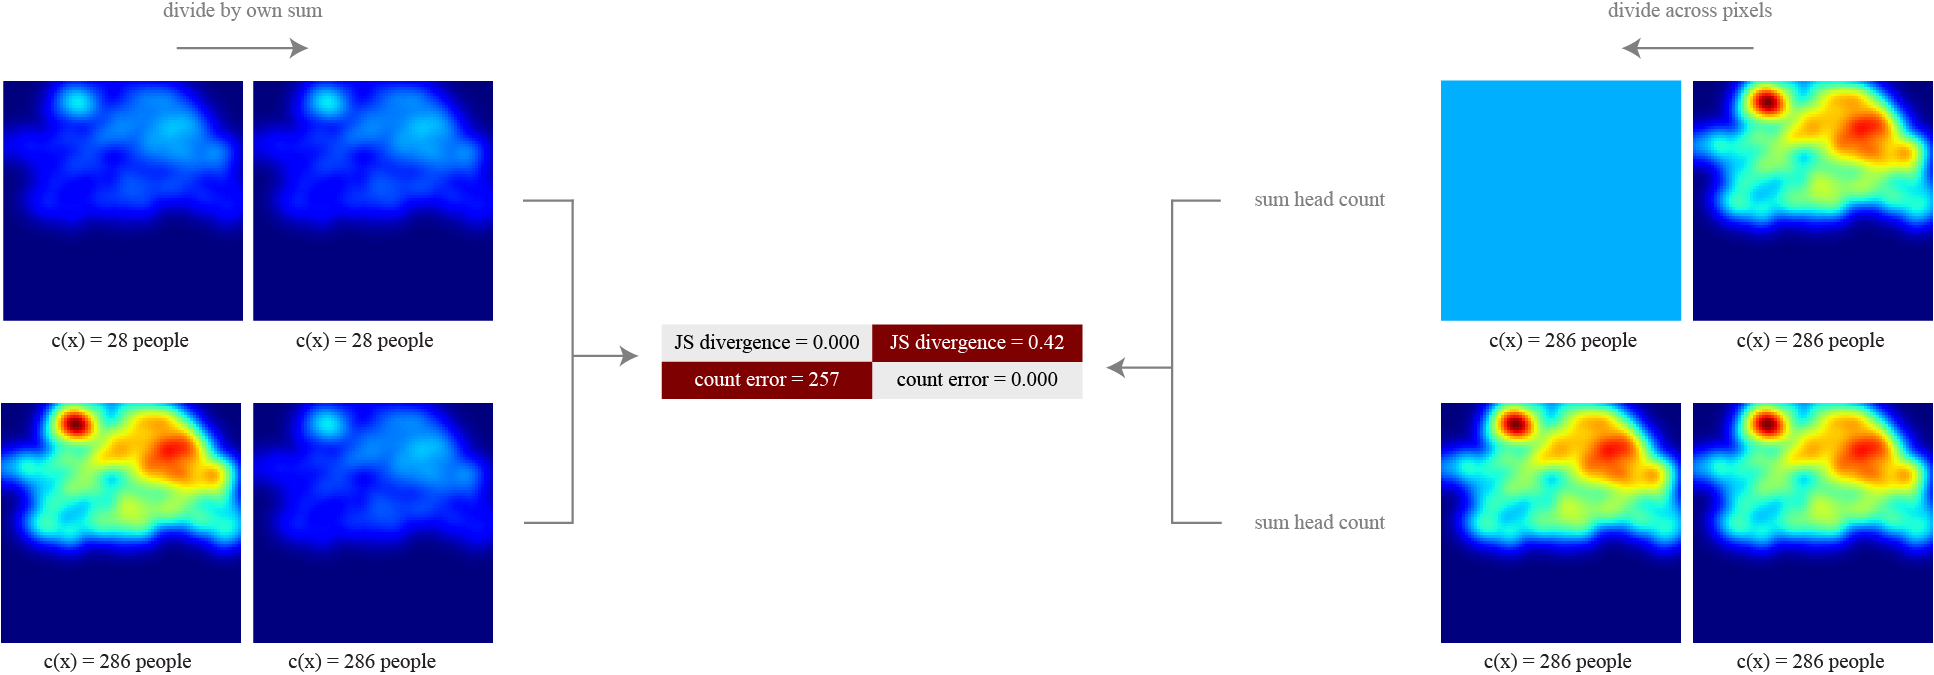
\includegraphics[width=\textwidth]{figs/Problem.png}
  \caption{Count and placement can fail separately. Left: a GCS frame and the same arrangement at one tenth the density have zero JS divergence after normalization, despite a headcount error of 257 people. Right: a uniform map with the true headcount has zero count error and placement divergence $0.42$.}
  \label{fig:problem}
\end{figure*}

\subsection{Crowd Density Maps Are Mass}
\label{sec:motivation-mass}

A density map $x \in \mathbb{R}^{H \times W}_{\geq 0}$ sums unit-mass Gaussians at annotated heads \cite{lempitsky2010}, so $c(x) = \sum_{i,j} x_{ij}$ is its headcount. For a nonempty map, $x = c(x)\,\hat{x}$ with $\hat{x} = x / c(x)$: $c(x)$ gives the count and $\hat{x}$ the arrangement. Measuring both requires keeping the original scale.

Placement also has a distance. Predicting a crowd one cell away should differ from placing it across the concourse. Transport expresses this as $\sum_{p,q} \pi_{pq}\, d(p,q)$, where $\pi$ matches mass between maps and $d$ is distance on the image grid. Binwise divergence does not encode that distance.

The totals can differ too. People enter and leave the scene: $c(x_t) = 95$ may be followed by $c(x_{t+h}) = 130$. A forecast that misses this change is short by thirty-five people. If two maps have unequal totals, no plan satisfies both $\pi \mathbf{1} = x$ and $\pi^\top \mathbf{1} = y$. The comparison must allow unmatched mass and assign it a cost.

\subsection{Joint Count and Placement Error}
\label{sec:motivation-uot}

We use unbalanced optimal transport \cite{chizat2018, peyre2019}:

\begin{equation}
\label{eq:dkappa}
D_\kappa(x, y) = \underbrace{\sum_{p,q} \pi_{pq}\, d(p,q)}_{\text{transport}} \;+\; \kappa \underbrace{\left( \|x - \pi \mathbf{1}\|_1 + \|y - \pi^\top \mathbf{1}\|_1 \right)}_{\text{unmatched}},
\end{equation}

minimized over plans $\pi$. Transport is measured in people times pixels; unmatched mass is measured in people. The exchange rate $\kappa$ prices one unmatched person in pixels of displacement. Both terms come from the same plan and can be reported with the total.

We fix $\kappa = 8$ before examining results. On GCS, the pooled score is $50.6\%$ transport and $49.4\%$ unmatched mass. In the surge stratum the split is $47.5/52.5$. These are observed shares, not a balance imposed by the formulation.

The unmatched term depends on placement as well as count: mass can be left unmatched when transporting it is too costly. It therefore differs from the absolute difference between map totals in Equation~\ref{eq:countmae}. This distinction matters in sparse maps, where a shortfall of fifty people can be spread across 6{,}400 cells and contribute little to a pixel loss.

\subsection{Debiasing and Runtime}
\label{sec:motivation-computation}

Entropic regularization introduces a bias \cite{cuturi2013}. An initial diagnostic at $\varepsilon = 0.5$ and $\text{pool} = 2$ gave $D_\kappa = 10.51$ for a map compared with itself, with a nonzero gradient. Stream-CDF training therefore uses the debiased form $D_\kappa(x,y) - \tfrac{1}{2} D_\kappa(x,x) - \tfrac{1}{2} D_\kappa(y,y)$ \cite{feydy2019}, which is zero when the maps agree. The reported evaluation scores use the raw transport-plus-unmatched value without subtracting the self-comparisons, preserving the decomposition in Equation~\ref{eq:decomposition}.

Each frame is an independent transport problem, so frames from all clips can be processed in one batched Sinkhorn loop. Evaluating 1{,}448 clips takes seconds at $\varepsilon = 0.25$, 60 iterations, full resolution and double precision. Maps use a fixed storage scale; the unmatched term divides it out to remain in people.

This answers RQ2: one solve scores count and placement jointly, and batching makes it practical for this test set.

\section{Experimental Protocol}
\label{sec:experimental-setup}

\subsection{Datasets and Forecasting Clips}
\label{sec:setup-data}

We use the dense, dynamic Grand Central Station recording. It is supplied in scene blocks at 1.25\,fps. We follow the prior split, holding out eight blocks for testing. Each frame is an $80 \times 80$ density map, formed by summing isotropic Gaussians with $\sigma = 3$ grid cells at annotated heads. Maps retain their headcount and are stored at $100\times$ people; the metric divides out this scale.

Each clip contains $T = 8$ observed frames and $H = 12$ future frames: $6.4$\,s of observation and a $9.6$\,s forecast on GCS. Clips start at every frame offset and stay within block boundaries, giving 1{,}448 test clips. A second, indoor recording uses the same clip construction and gives 361 test clips.

\subsection{Crowd-Dynamics Stratification}
\label{sec:setup-strata}

We group clips by the range of their true headcount over the forecast horizon:

\begin{equation}
\label{eq:stratum}
s = \max_h c(y_{T+h}) - \min_h c(y_{T+h}),
\end{equation}

Quartiles define four roughly equal strata: \emph{flat}, \emph{moderate}, \emph{dynamic} and \emph{surge}. The GCS thresholds are $8.0$, $10.8$ and $15.3$ people. The range captures both growth and dispersal; on GCS, the surge stratum is mostly dispersal after train departures. Thresholds are computed separately for each recording, so matching stratum names do not imply matching crowd dynamics.

\subsection{Evaluation Metrics and UOT Configuration}
\label{sec:setup-metrics}

We fix $\kappa = 8$. Stream-CDF training uses $\varepsilon = 2.0$, 30 iterations and $\text{pool} = 2$ with the debiased objective. Evaluation uses $\varepsilon = 0.25$, 60 iterations, no pooling and double precision, and reports the raw transport-plus-unmatched value. Thus training and evaluation differ in both solver settings and the self-comparison subtraction. All reported prediction scores use the evaluation setting.

Tables~\ref{tab:gcs} and~\ref{tab:indoor} report five quantities from the same predictions. The primary score decomposes as

\begin{equation}
\label{eq:decomposition}
D_\kappa = \underbrace{T}_{\text{transport}} + \kappa \cdot \underbrace{u}_{\text{unmatched}},
\end{equation}

where $T$ is transport cost on the evaluation grid and $u$ is unmatched mass in people. Read the terms together: leaving mass unmatched avoids transport, so a smaller transport term alone need not mean better placement.

countMAE measures only the difference in totals:

\begin{equation}
\label{eq:countmae}
\mathrm{countMAE} = \frac{1}{H} \sum_{h=1}^{H} \left| c(\hat{y}_{T+h}) - c(y_{T+h}) \right|,
\end{equation}

It is expressed in people and ignores placement. $\mathrm{AD_{JS}}$ uses CrowdMAC's reference JS computation, averaged over the $H$ forecast steps:

\begin{equation}
\label{eq:adjs}
\mathrm{AD_{JS}} = \frac{1}{H} \sum_{h=1}^{H} \mathrm{JS}_{\mathrm{ref}}\!\left( y_{T+h}, \hat{y}_{T+h} \right),
\end{equation}

We use the published implementation \cite{fujii2025}, expressed in nats. It first forms $m = (x+y)/2$ from the unnormalized maps, then computes $\mathrm{JS}_{\mathrm{ref}}(x,y) = \tfrac{1}{2}\mathrm{KL}(\tilde{x}\,\|\,\tilde{m}) + \tfrac{1}{2}\mathrm{KL}(\tilde{y}\,\|\,\tilde{m})$, where each tilde denotes normalization by that map's own sum, up to the implementation's numerical safeguards. This differs from standard JS between independently normalized maps: the mixture can depend on relative counts when shapes differ, so the score is not universally a pure-shape measure and the standard $\ln 2$ bound does not apply. Proportional maps still receive the perfect-forecast score regardless of their headcount ratio.

\subsection{Forecasting Methods}
\label{sec:setup-methods}

We compare five learned, statistical and trivial forecasters to examine how the measures assess the same predictions.

\begin{figure*}[t]
  \centering
  \includegraphics[width=\textwidth]{figs/Forecaster.png}
  \caption{Forecaster architecture. Eight observed frames ($6.4$\,s on GCS) are cube-embedded and summarised into memory by a causal encoder; a horizon decoder cross-attends learned per-tubelet queries into that memory and emits twelve forecast frames ($9.6$\,s on GCS) as a residual on an anchor built from the last four observed frames.}
  \label{fig:forecaster}
\end{figure*}

\paragraph{Stream-CDF.} Our forecaster provides a learned comparison (Figure~\ref{fig:forecaster}). It embeds cubes of 4 frames by $8 \times 8$ cells, following video tubelet embedding \cite{tong2022videomae}, into 256 dimensions. Each time chunk has 100 spatial positions; $T = 8$ gives two chunks and $N = 200$ tokens. Four causal pre-norm transformer blocks with 4 heads encode them into memory. Learned queries cross-attend to this memory and decode the horizon in one pass, following the set-prediction decoder of \cite{carion2020detr}. Output tubelets span 2 frames, giving six tubelets over the twelve-frame horizon.

\paragraph{Persistence.} Repeats the last observed frame across the horizon. It has no parameters and is a strong baseline when the scene changes little.

\paragraph{CrowdMAC.} Reproduced from the published recipe \cite{fujii2025}, using the same clips, splits and maps. Its reported divergence is the metric examined here.

\paragraph{Holt + last.} Fits Holt's linear trend method \cite{holt2004} to observed counts, then distributes each forecast count over the normalized last observed frame.

\paragraph{Holt + uniform.} Uses the same Holt count forecast but distributes it evenly over the scene. The Holt pair has identical countMAE by construction, isolating the effect of placement.

\subsection{Implementation and Training Details}
\label{sec:setup-training}

Stream-CDF is trained on the debiased objective without an auxiliary loss for 20 epochs on GCS and 40 epochs indoors using AdamW: learning rate $2.5 \times 10^{-4}$, weight decay $10^{-4}$ on the weight-decay parameter group, batch size 8, cosine annealing and gradient-norm clipping at 750. The density head uses a fixed output gain of 10, a tanh residual bound of 50 in the stored density units, and a softplus output activation; its parameter group uses a 500-step linear warmup. The reported Stream-CDF predictions use final-epoch checkpoints rather than checkpoints selected by test error. Since count is the sum of the map, this loss supervises headcount without a separate output.

The reported runs use learned absolute temporal embeddings. The implementation also provides an optional replacement with the linear attention bias of Press et al. \cite{press2022alibi}:

\begin{equation}
\label{eq:alibi}
b_{h,ij} =
\begin{cases}
-\infty, & \tau(j) > \tau(i), \\
-m_h \left( \tau(i) - \tau(j) \right), & \text{otherwise,}
\end{cases}
\end{equation}

Here $m_h$ is fixed per head. The first case enforces causality; the second reduces attention with age. The bias depends on relative chunk distance, so it remains defined as a stream grows. Spatial positions keep their learned table. This optional bias is not used in the reported runs. Our evaluation uses fixed windows with absolute temporal embeddings; it does not test incremental KV caching or establish a benefit from longer context.

\section{Results}
\label{sec:results}

All prediction scores use the evaluation setting on the same 1{,}448 GCS and 361 indoor test clips.

\subsection{Controlled Failure Cases}
\label{sec:results-controlled}

\paragraph{Magnitude scaling.} Multiplying a true clip by 100 keeps its arrangement and replaces 45 people with 4{,}500. Against the original clip, $\mathrm{AD_{JS}} = -4.7 \times 10^{-7}$, the score of a perfect forecast to seven decimal places. The other five AD*/FD* measures also return the perfect-forecast score. This answers RQ1: normalization removes headcount error in the reference implementation.

\paragraph{Correct count, wrong placement.} A uniform map with the true headcount has zero count error despite losing the crowd's arrangement. Figure~\ref{fig:problem} gives both examples: the normalized 28-person and 286-person maps have $D_{\mathrm{JS}} = 0.000$ despite a count error of 257; the uniform map has count error $= 0.000$ and placement divergence $0.42$. Holt + uniform is a working forecast with this second failure.

\subsection{Metric Choice Changes Model Assessment}
\label{sec:results-reversal}

\begin{figure*}[t]
  \centering
  \includegraphics[width=\textwidth]{figs/pooled.png}
  \caption{Pooled countMAE, $D_\kappa$ and unmatched mass for all five forecasters, GCS (top) and indoor (bottom), $\kappa = 8$. GCS bars are the \emph{all} row of Table~\ref{tab:gcs}.}
  \label{fig:pooled}
\end{figure*}

\begin{table*}[t]
  \centering
  \small
  \setlength{\tabcolsep}{6pt}
  \begin{tabular}{llrrrrr}
    \toprule
    \textbf{stratum} & \textbf{model} & countMAE & \multicolumn{3}{c}{$D_\kappa$ decomposition} & ADJS \\
    \cmidrule(lr){4-6}
     &  & \scriptsize\emph{pure count} & $D_\kappa$ & unmatched & transport & \scriptsize\emph{reference JS} \\
    \midrule
    \emph{flat} ($n=363$) & Stream-CDF & 3.59 & \textbf{203.3} & \textbf{12.01} & 107.2 & 0.1446 \\
     & persistence & \textbf{3.27} & 209.6 & 12.45 & 110.0 & \textbf{0.0818} \\
     & CrowdMAC & 5.49 & 293.0 & 19.42 & 137.7 & 0.1087 \\
     & Holt + last & 8.72 & 222.9 & 15.13 & \textbf{101.9} & 0.0836 \\
     & Holt + uniform & 8.72 & 615.4 & 63.27 & 109.3 & 0.2919 \\
    \midrule
    \emph{moderate} ($n=361$) & Stream-CDF & 4.41 & \textbf{228.4} & \textbf{13.51} & 120.3 & 0.1274 \\
     & persistence & \textbf{4.22} & 235.7 & 13.98 & 123.9 & \textbf{0.0719} \\
     & CrowdMAC & 7.17 & 333.5 & 22.19 & 155.9 & 0.0979 \\
     & Holt + last & 9.86 & 252.4 & 16.92 & \textbf{117.0} & 0.0740 \\
     & Holt + uniform & 9.86 & 729.4 & 75.65 & 124.2 & 0.2879 \\
    \midrule
    \emph{dynamic} ($n=363$) & Stream-CDF & 6.00 & \textbf{258.0} & \textbf{15.73} & 132.2 & 0.1070 \\
     & persistence & \textbf{5.82} & 264.4 & 16.07 & 135.9 & \textbf{0.0594} \\
     & CrowdMAC & 8.31 & 374.7 & 24.52 & 178.6 & 0.0872 \\
     & Holt + last & 10.26 & 280.5 & 18.71 & \textbf{130.8} & 0.0639 \\
     & Holt + uniform & 10.26 & 861.4 & 89.89 & 142.3 & 0.2848 \\
    \midrule
    \emph{surge} ($n=361$) & Stream-CDF & 10.63 & \textbf{335.6} & \textbf{22.05} & 159.3 & 0.0808 \\
     & persistence & \textbf{10.39} & 341.8 & 22.37 & 162.9 & \textbf{0.0452} \\
     & CrowdMAC & 28.25 & 570.7 & 43.68 & 221.3 & 0.0790 \\
     & Holt + last & 14.19 & 358.1 & 25.01 & \textbf{158.0} & 0.0454 \\
     & Holt + uniform & 14.19 & 1268.4 & 134.35 & 193.6 & 0.2730 \\
    \midrule
    \emph{all} ($n=1448$) & Stream-CDF & 6.16 & \textbf{256.3} & \textbf{15.82} & 129.7 & 0.1150 \\
     & persistence & \textbf{5.92} & 262.8 & 16.21 & 133.1 & \textbf{0.0646} \\
     & CrowdMAC & 12.29 & 392.8 & 27.44 & 173.3 & 0.0932 \\
     & Holt + last & 10.75 & 278.4 & 18.94 & \textbf{126.9} & 0.0667 \\
     & Holt + uniform & 10.75 & 868.3 & 90.75 & 142.3 & 0.2844 \\
    \bottomrule
  \end{tabular}
  \caption{Results on 1{,}448 GCS test clips, $\kappa = 8$. Bold marks the lowest value per column within each stratum. $D_\kappa = \text{transport} + \kappa \cdot \text{unmatched}$, with unmatched mass in people; ADJS is horizon-averaged Jensen--Shannon divergence. Transport and unmatched mass trade off, so lower transport alone need not mean better placement. The \emph{all} row pools the test set. Stratum thresholds differ from Table~\ref{tab:indoor}.}
  \label{tab:gcs}
\end{table*}

The same predictions give different rankings in Table~\ref{tab:gcs}. On the pooled row, countMAE favors persistence (5.92), followed by Stream-CDF (6.16), the tied Holt variants (10.75), and CrowdMAC (12.29). $\mathrm{AD_{JS}}$ orders them as persistence (0.0646), Holt + last (0.0667), CrowdMAC (0.0932), Stream-CDF (0.1150), and Holt + uniform (0.2844). Under $D_\kappa$, Stream-CDF comes first (256.3), then persistence (262.8), Holt + last (278.4), CrowdMAC (392.8), and Holt + uniform (868.3).

Stream-CDF is fourth under normalized divergence and first under $D_\kappa$ in every GCS stratum. For RQ3, the ranking change therefore survives the dynamics split; it is not an effect of pooling clips from different regimes.

The Holt pair shows why count alone is insufficient. Both variants have the same countMAE in every stratum, yet their pooled $D_\kappa$ differs by a factor of $3.1$ (278.4 against 868.3). Most of the gap is unmatched mass: 18.94 against 90.75 people, compared with transport costs of 126.9 and 142.3. A correct total can still be costly when placed across the wrong cells.

This also explains why countMAE and unmatched mass disagree. countMAE puts CrowdMAC last, while unmatched mass puts Holt + uniform last (90.75 against 27.44 people pooled). The latter depends on what can be matched under the transport plan, not just the difference in totals.

\subsection{Performance Across Crowd-Dynamics Regimes}
\label{sec:results-strata}

\begin{figure*}[t]
  \centering
  \includegraphics[width=\textwidth]{figs/stratified.png}
  \caption{countMAE, $D_\kappa$ and unmatched mass by ground-truth dynamic level, GCS (top) and indoor (bottom). The two Holt variants share a count forecast and coincide on countMAE by construction.}
  \label{fig:stratified}
\end{figure*}

Every GCS forecaster's countMAE and $D_\kappa$ rise as the crowd changes more (Figure~\ref{fig:stratified}). Pooled scores sit near the \emph{dynamic} stratum and understate error during \emph{surge}.

The size of that change differs by model. Surge-to-pooled $D_\kappa$ ratios range from $1.29$ to $1.46$. For countMAE, four models range from $1.32$ to $1.76$, while CrowdMAC reaches $2.30$. Its count error rises from 8.31 in \emph{dynamic} to 28.25 in \emph{surge}, against a pooled 12.29. The pooled count error is roughly twice Stream-CDF's; in surge it is nearly three times as large. This is the second part of the answer to RQ3: the pooled row hides how sharply a model fails when the crowd changes.

The joint score softens this particular failure because its transport term grows more slowly than count error. CrowdMAC's unmatched mass rises from 24.52 to 43.68 people between dynamic and surge. Reporting the decomposition preserves that information; the total alone is insufficient.

\subsection{Sensitivity to $\kappa$}
\label{sec:results-kappa}

\begin{figure}[t]
  \centering
  \includegraphics[width=.75\columnwidth]{figs/kappasweep.png}
  \caption{$D_\kappa$ (solid, left axis) and its transport share (dotted, right axis) as $\kappa$ ranges from $0.5$ to $64$, on GCS (top) and indoor (bottom). Circles mark rank crossovers among Stream-CDF, persistence and Holt + last. Main results use $\kappa = 8$.}
  \label{fig:kappasweep}
\end{figure}

Figure~\ref{fig:kappasweep} sweeps $\kappa$ from $0.5$ to $64$. At low values, unmatched mass is cheap, and the order of Stream-CDF, persistence and Holt + last changes. Crossovers occur below $\kappa \approx 2$ on GCS and below $\kappa \approx 11$ indoors. Above those thresholds their order holds through $\kappa = 64$. CrowdMAC and Holt + uniform remain outside this group throughout the sweep.

The chosen $\kappa = 8$ lies in the stable GCS range, supporting the reversal reported there. The indoor crossover range extends beyond this value, so the sweep does not support the same stability claim indoors.

\subsection{Qualitative Analysis}
\label{sec:results-qualitative}

\begin{figure*}[t]
  \centering
  \begin{subfigure}[t]{0.48\textwidth}
    \centering
    \includegraphics[width=\linewidth]{figs/CDF vs GT.png}
    \caption{Dispersal}
    \label{fig:qualitative-dispersal}
  \end{subfigure}
  \hfill
  \begin{subfigure}[t]{0.48\textwidth}
    \centering
    \includegraphics[width=\linewidth]{figs/CDF vs GT - 2.png}
    \caption{Growth}
    \label{fig:qualitative-growth}
  \end{subfigure}
  \caption{Ground truth, Stream-CDF and Holt + uniform predictions at $t{+}1, t{+}3, t{+}5, t{+}7$ for two GCS clips. Counts are annotated per panel; Holt + uniform's count tracks the ground truth as closely as Stream-CDF's while carrying no spatial information.}
  \label{fig:qualitative}
\end{figure*}

Figure~\ref{fig:qualitative} compares two GCS clips at $t{+}1, t{+}3, t{+}5, t{+}7$. Stream-CDF preserves the two main clusters and tracks the true count within a few people. Its visible checkerboard comes from cube boundaries. Holt + uniform matches or beats its count at every shown step, but spreads the crowd over the whole frame. The totals look similarly accurate; the maps give different answers about where the crowd will be.

\subsection{Cross-Recording Evaluation}
\label{sec:results-indoor}

\begin{table}[t]
  \centering
  \small
  \setlength{\tabcolsep}{6pt}
  \begin{tabular}{llrrrrr}
    \toprule
    \textbf{stratum} & \textbf{model} & countMAE & \multicolumn{3}{c}{$D_\kappa$ decomposition} & ADJS \\
    \cmidrule(lr){4-6}
     &  & \scriptsize\emph{pure count} & $D_\kappa$ & unmatched & transport & \scriptsize\emph{reference JS} \\
    \midrule
    \emph{flat} ($n=92$) & Stream-CDF & 5.51 & 79.4 & 7.54 & 19.1 & 0.0904 \\
     & persistence & \textbf{4.70} & \textbf{75.5} & \textbf{7.17} & 18.1 & \textbf{0.0460} \\
    \midrule
    \emph{moderate} ($n=93$) & Stream-CDF & 5.35 & \textbf{87.6} & \textbf{7.86} & 24.7 & 0.0921 \\
     & persistence & 5.75 & 88.3 & 8.33 & 21.7 & \textbf{0.0370} \\
    \midrule
    \emph{dynamic} ($n=87$) & Stream-CDF & \textbf{5.07} & \textbf{81.6} & \textbf{7.37} & 22.6 & 0.0820 \\
     & persistence & 5.73 & 82.1 & 7.95 & 18.5 & \textbf{0.0299} \\
    \midrule
    \emph{surge} ($n=89$) & Stream-CDF & \textbf{5.39} & 80.6 & \textbf{7.35} & 21.8 & 0.0685 \\
     & persistence & 6.02 & \textbf{80.2} & 7.73 & 18.4 & \textbf{0.0259} \\
    \midrule
    \emph{all} ($n=361$) & Stream-CDF & \textbf{5.34} & 82.3 & \textbf{7.53} & 22.1 & 0.0834 \\
     & persistence & 5.54 & \textbf{81.5} & 7.79 & 19.2 & \textbf{0.0348} \\
    \bottomrule
  \end{tabular}
  \caption{Results on 361 indoor test clips, $\kappa = 8$, for Stream-CDF and persistence. Figure~\ref{fig:pooled} shows all five forecasters pooled. Bold marks the lowest value per column within each stratum. Columns follow Table~\ref{tab:gcs}; stratum thresholds are computed separately for this recording.}
  \label{tab:indoor}
\end{table}

The full GCS reordering does not transfer indoors. Table~\ref{tab:indoor} focuses on Stream-CDF and persistence; Figure~\ref{fig:pooled} includes all five models. CrowdMAC ranks last under both measures in every indoor stratum.

Normalized divergence favors persistence throughout. Under $D_\kappa$, Stream-CDF is slightly better in moderate and dynamic clips, while persistence is better in flat, surge and pooled results. The pooled scores are 82.3 and 81.5, respectively. Stream-CDF has lower pooled countMAE (5.34 against 5.54) and unmatched mass (7.53 against 7.79), but higher transport cost (22.1 against 19.2). The measures still disagree, though these small gaps do not establish a reliable model ranking.

\section{Limitations}
\label{sec:limitations}

We study two recordings, and the consistent ranking reversal appears only on GCS. One concourse is a narrow basis for generalization. The indoor recording shows disagreement between measures, with smaller differences and a different ordering.

The fixed $\kappa = 8$ is not calibrated to an operational cost. It gives transport $50.6\%$ of the pooled GCS score and unmatched mass $49.4\%$; transport contributes only $24$--$27\%$ indoors. Camera geometry and frame rate may require a different exchange rate. Calibrating it from walking speed or an operator's tolerance for count error remains open.

We have not tested whether the joint score improves an alert or matches an operator's preference. That requires a downstream decision, as decision-based verification in related forecasting tasks makes clear \cite{ravuri2021}.

Each forecaster has one run. The GCS reversal holds across all four strata, but this does not measure training variability. Several indoor $D_\kappa$ gaps are under one point and need repeated runs before supporting a ranking.

\section{Conclusion}
\label{sec:conclusion}

Normalized divergence removes the headcount carried by a density map. The controlled test confirms this in the reference implementation. Unbalanced transport keeps count and placement in one comparison and evaluates the test set in seconds. On GCS, that choice moves Stream-CDF from fourth to first in every dynamics stratum. Stratification also exposes CrowdMAC's larger count error during rapid change, while the indoor results limit how far the ranking can be generalized.

A crowd forecast needs to say how many people and where. Evaluation should keep both, and report where the forecast fails.


\bibliographystyle{unsrtnat}

{\small
\begin{thebibliography}{99}

\bibitem{alahi2016social}
Alexandre Alahi, Kratarth Goel, Vignesh Ramanathan, Alexandre Robicquet,
  Li Fei-Fei, and Silvio Savarese.
\newblock Social {LSTM}: Human trajectory prediction in crowded spaces.
\newblock In {\em IEEE Conference on Computer Vision and Pattern Recognition
  (CVPR)}, 2016.

\bibitem{chizat2018}
Lenaic Chizat, Gabriel Peyr\'e, Bernhard Schmitzer, and Fran\c{c}ois-Xavier
  Vialard.
\newblock Scaling algorithms for unbalanced optimal transport problems.
\newblock {\em Mathematics of Computation}, 87(314):2563--2609, 2018.

\bibitem{cuturi2013}
Marco Cuturi.
\newblock Sinkhorn distances: Lightspeed computation of optimal transport.
\newblock In {\em Advances in Neural Information Processing Systems (NeurIPS)},
  2013.

\bibitem{feydy2019}
Jean Feydy, Thibault S\'ejourn\'e, Fran\c{c}ois-Xavier Vialard, Shun-ichi
  Amari, Alain Trouv\'e, and Gabriel Peyr\'e.
\newblock Interpolating between optimal transport and {MMD} using {S}inkhorn
  divergences.
\newblock In {\em International Conference on Artificial Intelligence and
  Statistics (AISTATS)}, 2019.

\bibitem{holt2004}
Charles~C. Holt.
\newblock Forecasting seasonals and trends by exponentially weighted moving
  averages.
\newblock {\em International Journal of Forecasting}, 20(1):5--10, 2004.
\newblock Reprint of the 1957 Office of Naval Research memorandum.

\bibitem{peyre2019}
Gabriel Peyr\'e and Marco Cuturi.
\newblock Computational optimal transport.
\newblock {\em Foundations and Trends in Machine Learning}, 11(5-6):355--607,
  2019.

\bibitem{carion2020detr}
Nicolas Carion, Francisco Massa, Gabriel Synnaeve, Nicolas Usunier,
  Alexander Kirillov, and Sergey Zagoruyko.
\newblock End-to-end object detection with transformers.
\newblock In {\em European Conference on Computer Vision (ECCV)}, 2020.

\bibitem{das2024timesfm}
Abhimanyu Das, Weihao Kong, Rajat Sen, and Yichen Zhou.
\newblock A decoder-only foundation model for time-series forecasting.
\newblock In {\em International Conference on Machine Learning (ICML)}, 2024.

\bibitem{doublepenalty2025}
Christopher Subich, Syed Zahid Husain, Leo Separovic, and Jing Yang.
\newblock Fixing the double penalty in data-driven weather forecasting through a
  modified spherical harmonic loss function.
\newblock {\em arXiv preprint arXiv:2501.19374}, 2025.

\bibitem{fang2019fdst}
Yanyan Fang, Biyun Zhan, Wandi Cai, Shenghua Gao, and Bo Hu.
\newblock Locality-constrained spatial transformer network for video crowd
  counting.
\newblock In {\em IEEE International Conference on Multimedia and Expo (ICME)},
  2019.

\bibitem{fujii2025}
Ryo Fujii, Ryo Hachiuma, and Hideo Saito.
\newblock {CrowdMAC}: Masked crowd density completion for robust crowd density
  forecasting.
\newblock In {\em IEEE/CVF Winter Conference on Applications of Computer Vision
  (WACV)}, pages 8218--8227, 2025.

\bibitem{gupta2018socialgan}
Agrim Gupta, Justin Johnson, Li Fei-Fei, Silvio Savarese, and
  Alexandre Alahi.
\newblock Social {GAN}: Socially acceptable trajectories with generative
  adversarial networks.
\newblock In {\em IEEE Conference on Computer Vision and Pattern Recognition
  (CVPR)}, 2018.

\bibitem{lempitsky2010}
Victor Lempitsky and Andrew Zisserman.
\newblock Learning to count objects in images.
\newblock In {\em Advances in Neural Information Processing Systems (NeurIPS)},
  2010.

\bibitem{li2018}
Yuhong Li, Xiaofan Zhang, and Deming Chen.
\newblock {CSRNet}: Dilated convolutional neural networks for understanding the
  highly congested scenes.
\newblock In {\em IEEE Conference on Computer Vision and Pattern Recognition
  (CVPR)}, 2018.

\bibitem{ma2019}
Zhiheng Ma, Xing Wei, Xiaopeng Hong, and Yihong Gong.
\newblock Bayesian loss for crowd count estimation with point supervision.
\newblock In {\em IEEE/CVF International Conference on Computer Vision (ICCV)},
  2019.

\bibitem{minoura2020}
Hiroaki Minoura, Ryo Yonetani, Mai Nishimura, and Yoshitaka Ushiku.
\newblock Crowd density forecasting by modeling patch-based dynamics.
\newblock {\em IEEE Robotics and Automation Letters}, 2020.

\bibitem{morales2025}
Marcela Morales Quispe and Jean-Bernard Hayet.
\newblock Predicting crowd motion with diffusion models.
\newblock In {\em Mexican Conference on Pattern Recognition (MCPR)}, volume
  15715 of {\em Lecture Notes in Computer Science}, pages 373--384. Springer,
  2025.

\bibitem{mscdp2023}
Shuyu Wang, Yan Lyu, Yuhang Xu, and Weiwei Wu.
\newblock {MSCDP}: Multi-step crowd density predictor in indoor environment.
\newblock {\em Neurocomputing}, 2023.

\bibitem{namazi2026}
Alireza Namazi and Heman Shakeri.
\newblock From prediction to practice: A task-aware evaluation framework for
  blood glucose forecasting.
\newblock {\em arXiv preprint arXiv:2605.00645}, 2026.

\bibitem{niu2020}
Yuzhen Niu, Weifeng Shi, Wenxi Liu, Shengfeng He, Jia Pan, and
  Antoni~B. Chan.
\newblock Over-crowdedness alert! {F}orecasting the future crowd distribution.
\newblock {\em arXiv preprint arXiv:2006.05127}, 2020.

\bibitem{oakden2020}
Luke Oakden-Rayner, Jared Dunnmon, Gustavo Carneiro, and Christopher R\'e.
\newblock Hidden stratification causes clinically meaningful failures in machine
  learning for medical imaging.
\newblock In {\em ACM Conference on Health, Inference, and Learning (CHIL)},
  2020.

\bibitem{phungtua2026}
Thanapol Phungtua-eng and Yoshitaka Yamamoto.
\newblock Are we winning the wrong game? {R}evisiting evaluation practices for
  long-term time series forecasting.
\newblock {\em arXiv preprint arXiv:2603.08156}, 2026.

\bibitem{press2022alibi}
Ofir Press, Noah~A. Smith, and Mike Lewis.
\newblock Train short, test long: Attention with linear biases enables input
  length extrapolation.
\newblock In {\em International Conference on Learning Representations (ICLR)},
  2022.

\bibitem{ravuri2021}
Suman Ravuri, Karel Lenc, Matthew Willson, Dmitry Kangin, Remi Lam,
  Piotr Mirowski, Megan Fitzsimons, Maria Athanassiadou, Sheleem Kashem,
  Sam Madge, Rachel Prudden, Amol Mandhane, Aidan Clark, Andrew Brock,
  Karen Simonyan, Raia Hadsell, Niall Robinson, Ellen Clancy,
  Alberto Arribas, and Shakir Mohamed.
\newblock Skilful precipitation nowcasting using deep generative models of
  radar.
\newblock {\em Nature}, 597:672--677, 2021.

\bibitem{shi2015convlstm}
Xingjian Shi, Zhourong Chen, Hao Wang, Dit-Yan Yeung, Wai-Kin Wong, and
  Wang-chun Woo.
\newblock Convolutional {LSTM} network: A machine learning approach for
  precipitation nowcasting.
\newblock In {\em Advances in Neural Information Processing Systems (NeurIPS)},
  2015.

\bibitem{sundararaman2021crohd}
Ramana Sundararaman, Cedric De~Almeida~Braga, Eric Marchand, and
  Julien Pettre.
\newblock Tracking pedestrian heads in dense crowd.
\newblock In {\em IEEE/CVF Conference on Computer Vision and Pattern Recognition
  (CVPR)}, 2021.

\bibitem{tong2022videomae}
Zhan Tong, Yibing Song, Jue Wang, and Limin Wang.
\newblock {VideoMAE}: Masked autoencoders are data-efficient learners for
  self-supervised video pre-training.
\newblock In {\em Advances in Neural Information Processing Systems (NeurIPS)},
  2022.

\bibitem{vtcrowdnet2026}
C.~Z. Thomas Xie, Xiaoxia Yang, Y. Tian, et al.
\newblock Inferring crowd crush accidents in typical high-density pedestrian
  movement zones via the vision--trajectory fusion neural network.
\newblock {\em Accident Analysis \& Prevention}, 230, 2026.

\bibitem{wang2020}
Boyu Wang, Huidong Liu, Dimitris Samaras, and Minh Hoai.
\newblock Distribution matching for crowd counting.
\newblock In {\em Advances in Neural Information Processing Systems (NeurIPS)},
  2020.

\bibitem{wang2021}
Qi Wang, Junyu Gao, Wei Lin, and Xuelong Li.
\newblock {NWPU-Crowd}: A large-scale benchmark for crowd counting and
  localization.
\newblock {\em IEEE Transactions on Pattern Analysis and Machine Intelligence},
  43(6):2141--2149, 2021.

\bibitem{curvbench2026}
Shuo Wang, Xiangyu Wang, Quanxin Wang, Bailin Wu, Bokui Wang,
  Shunyang Huang, Boyan Deng, Haonan Liu, Ruiyi Fang, Zhenxiang Xu,
  Boyu Wang, and Zhao Kang.
\newblock The post-{GCN} decade revisited: Curvature-stratified evaluation of
  relational learning.
\newblock {\em arXiv preprint arXiv:2606.06397}, 2026.

\bibitem{wang2026}
Yingshuo Wang, Xian Sun, Lingdong Kong, Wei Gao, Yanhang Li,
  Zhichao Fan, and Zexin Zhuang.
\newblock Do time series foundation model benchmarks hide regime-dependent
  failures? {E}vidence from traffic speed forecasting.
\newblock In {\em ICML Workshop on Forecasting as a New Frontier of
  Intelligence}, 2026.

\bibitem{wuhanmetro}
Hao Lu, Xuhui Zhu, Wenjing Zhang, Yanan Li, and Xiang Bai.
\newblock Crowded video individual counting informed by social grouping and
  spatial-temporal displacement priors.
\newblock {\em arXiv preprint arXiv:2601.01192}, 2026.

\bibitem{event2017}
Cliceres Mack Dal~Bianco, Soraia Raupp Musse, Alessandro Braun,
  Rafael Peruzzo Caetani, Claudio~R. Jung, and Norman~I. Badler.
\newblock Predicting future crowd motion including event treatment.
\newblock In {\em Intelligent Virtual Agents (IVA)}, volume 10498 of
  {\em Lecture Notes in Computer Science}, pages 132--142. Springer, 2017.

\bibitem{zhang2016}
Yingying Zhang, Desen Zhou, Siqin Chen, Shenghua Gao, and Yi Ma.
\newblock Single-image crowd counting via multi-column convolutional neural
  network.
\newblock In {\em IEEE Conference on Computer Vision and Pattern Recognition
  (CVPR)}, pages 589--597, 2016.

\end{thebibliography}
}
\end{document}
